
\cmt{We rely on the workflow depicted in \fig{fig:workflow} to address the question raised in our contribution. The key stages of the process involve \emph{Modeling}, \emph{Simulation}, \emph{Learning}, and \emph{Verification}.}

\begin{figure*}[!htb]
    \centering
    		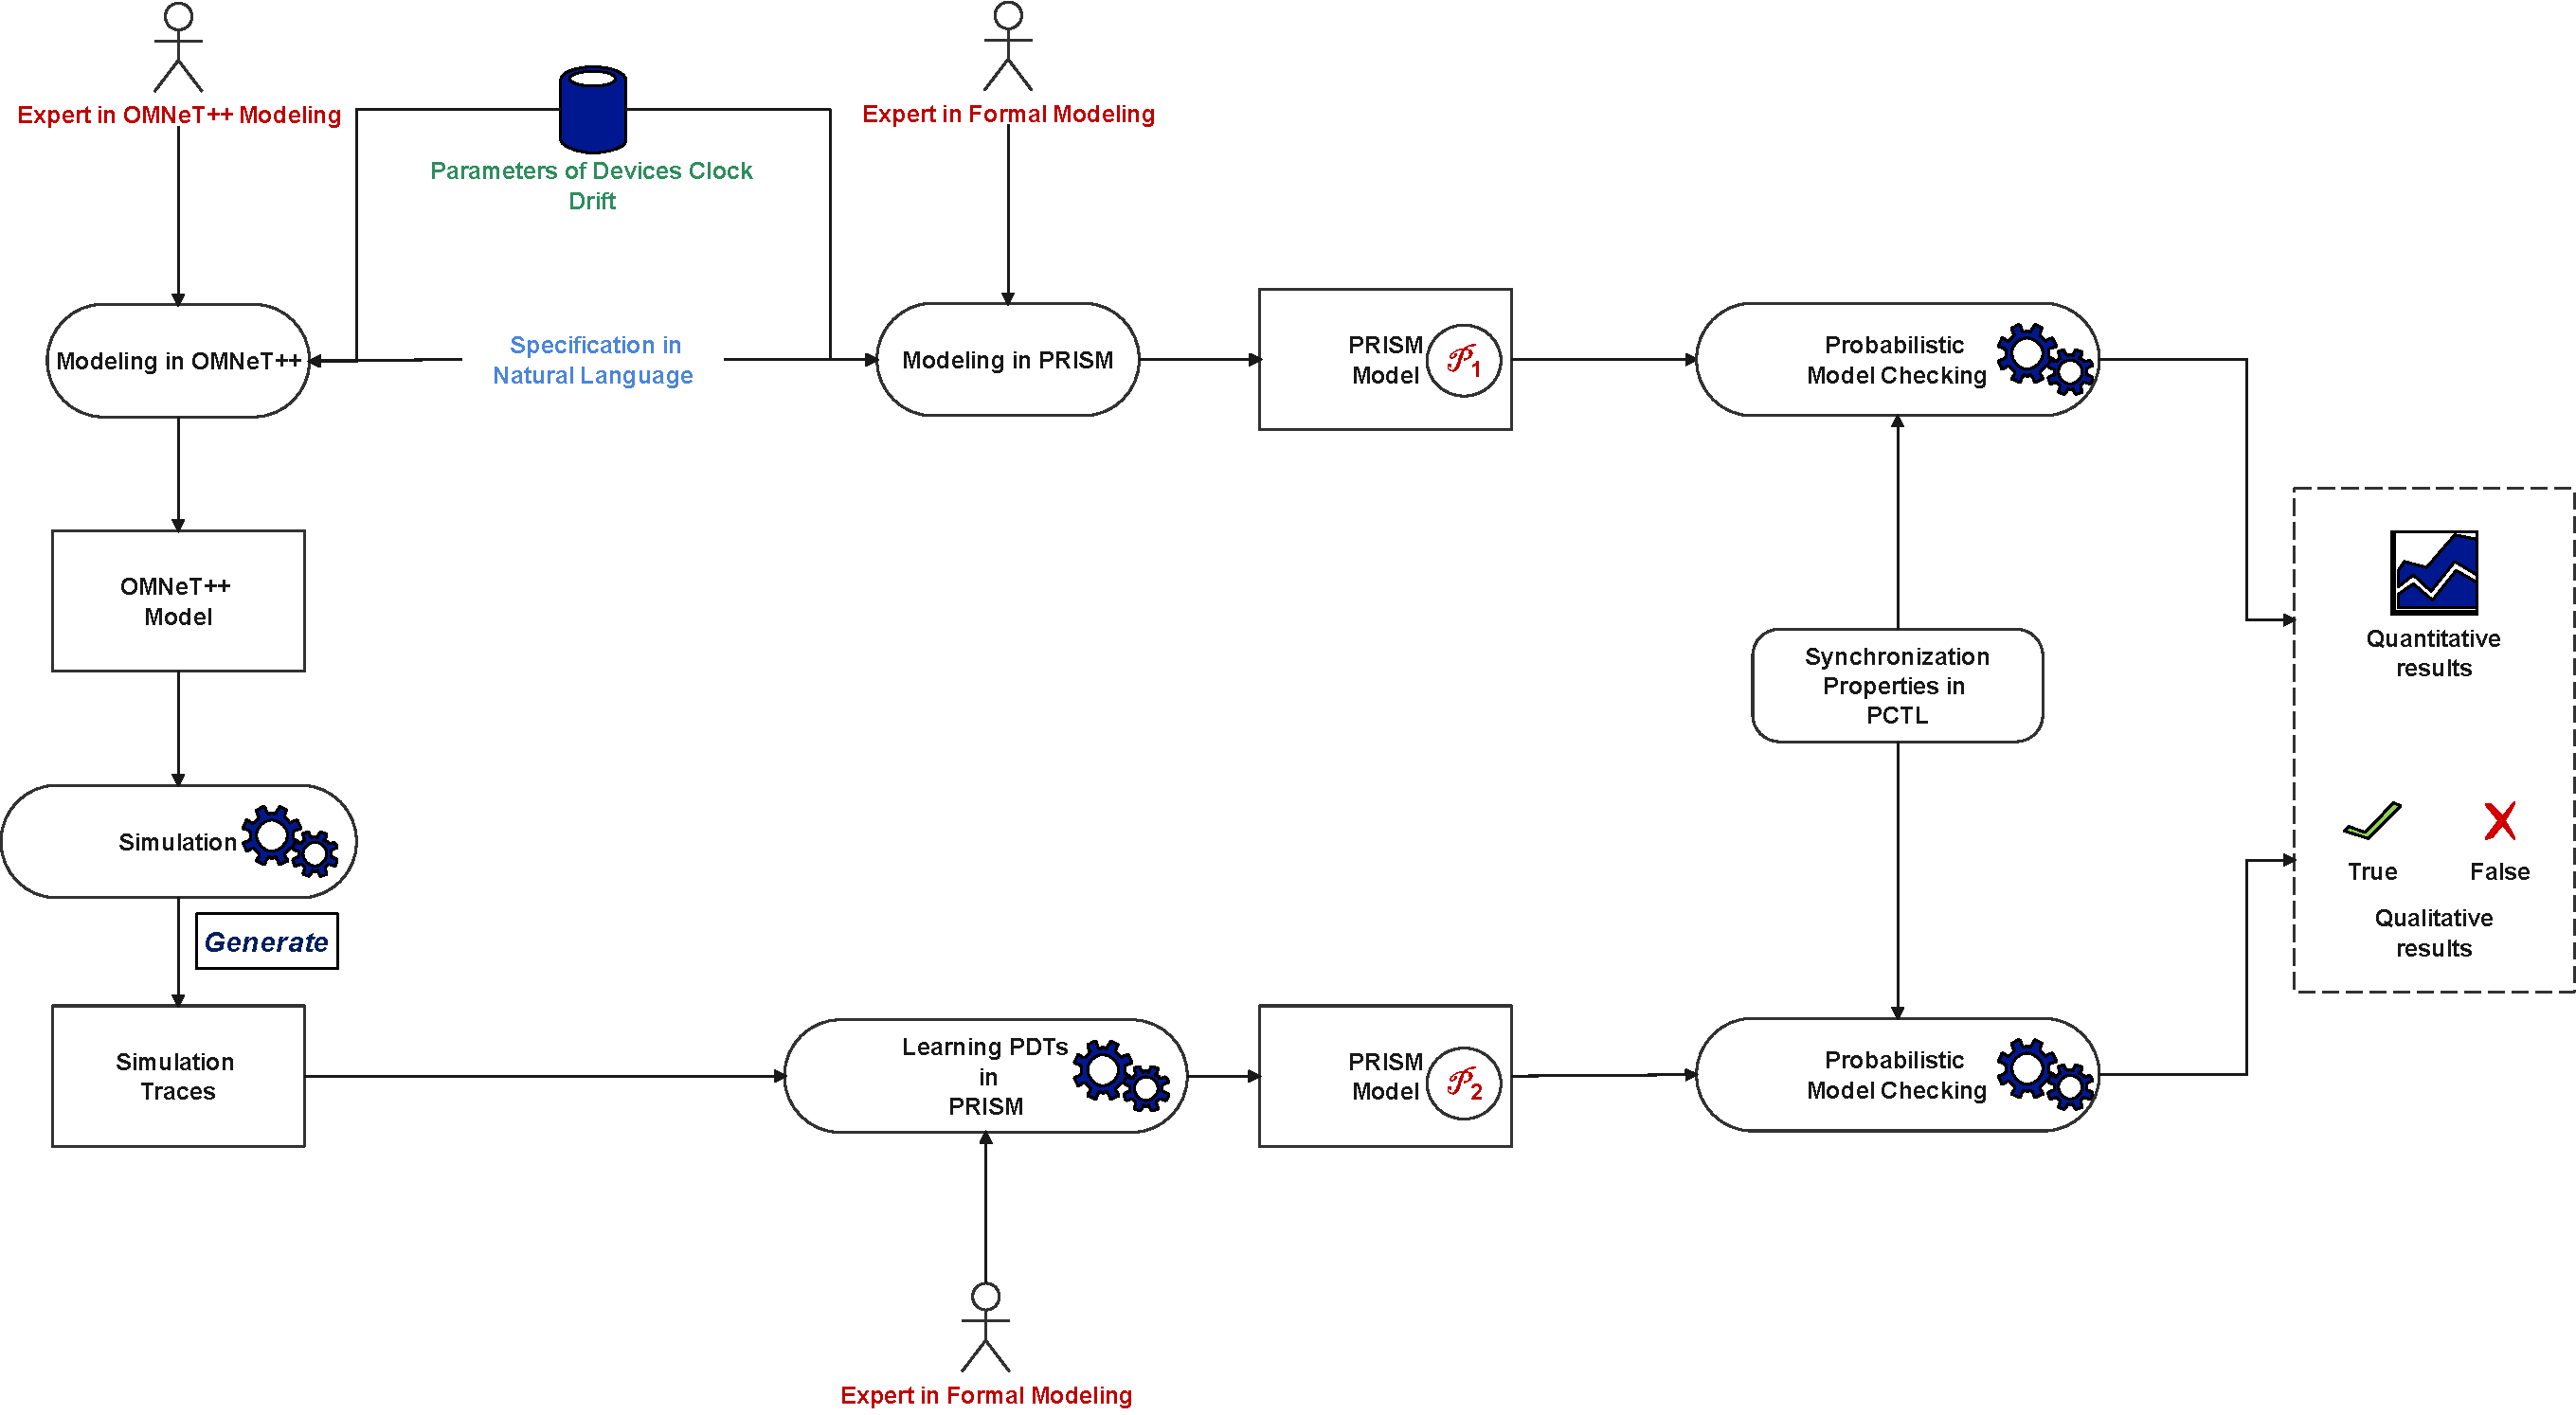
\includegraphics[width=460pt, height =270pt]{workflow.pdf}
    \caption{Proposed Flow for Verification and Validation.}
    \label{fig:workflow}
\end{figure*} 
\paragraph{Modeling} This specification uses natural language, making it easy for experts to model their existing system and identify clock frequencies from various sources. The modeled system is then translated into the PRISM language for verification using model-checking techniques (referred to as \emath{\mathcal{P}_{1}}). An OMNeT++ model is also built based on a natural language specification using C/C++ constructs. 

\paragraph{Simulation} The OMNeT ++ model was then simulated within the OMNeT++ graphical simulator. This simulation generates a set of traces to evaluate the timing and synchronization behavior of the system.



\paragraph{Learning} PDT is generated by learning from the traces collected from the OMNeT++ simulator. The learned PDT is then transformed into a new PRISM model \emath{\mathcal{P}_{2}}.

\paragraph{Verification} Finally, we evaluate the reliability of the synchronization planned by the PRISM models (M1 and M2) by checking them against system properties expressed in Probabilistic Computation Tree Logic (PCTL). We will also discuss some verification outcomes related to the scalability of the model \emath{\mathcal{P}_{2}}.

%{\bf BH: To continue from here}
%We will discuss some verification outcomes regarding scalability.
